\chapter{Matrix \cite{mfml-1}}\label{chapter: Matrix}

\section*{Intro \cite{mfml-1}}

With $m, n \in \mathbb{N}$ a real-valued $(m, n)$-matrix $\mathbf{A}$ is an $m\cdot n$-tuple of elements $a_{ij}$, $i = 1, \cdots , m$, $j = 1, \cdots , n$, which is ordered according to a rectangular scheme consisting of $m$ rows and $n$ columns:
\[
    \hfill
    \mathbf{A} = \begin{bmatrix}
        a_{11} & a_{12} & \cdots & a_{1n}\\
        a_{21} & a_{22} & \cdots & a_{2n}\\
        \vdots & \vdots & \ddots & \vdots\\
        a_{m1} & a_{m2} & \cdots & a_{mn}\\
    \end{bmatrix}
    \in \mathbb{R}^{m\times n}
    \hfill
\]

\begin{enumerate}
    \item $\mathbb{R}^{m\times n}$ is the set of all real-valued $(m, n)$-matrices

    \item (\textbf{flattening}) $\mathbf{A} \in \mathbb{R}^{m\times n}$ (matrix) can be equivalently represented as $\mathbf{a} \in \mathbb{R}^{mn\times 1}$ (vector) by stacking all $n$ columns of the matrix into a long vector
\end{enumerate}


\section{Matrix Addition ( $\mathbf{A + B}$ ) \cite{mfml-1}}\label{Matrix Addition}
The sum of two matrices $\mathbf{A, B} \in \mathbb{R}^{m\times n}$ is defined as the element-wise sum:
\[
    \hfill
    \mathbf{A + B} = \begin{bmatrix}
        a_{11} + b_{11} & a_{12} + b_{12} & \cdots & a_{1n} + b_{1n}\\
        a_{21} + b_{21} & a_{22} + b_{22} & \cdots & a_{2n} + b_{2n}\\
        \vdots & \vdots & \ddots & \vdots\\
        a_{m1} + b_{m1} & a_{m2} + b_{m2} & \cdots & a_{mn} + b_{mn}\\
    \end{bmatrix}
    \in \mathbb{R}^{m\times n}
    \hfill
\]


\section{Matrix Multiplication ( $AB = A@B$ ) \cite{mfml-1}}
For matrices $\mathbf{A} \in \mathbb{R}^{m\times n}$, $\mathbf{B} \in \mathbb{R}^{n\times k}$, the elements $c_{ij}$ of the product $C = AB = A@B \in \mathbb{R}^{m\times k}$ are computed as:
\[
    \displaystyle
    c_{ij} = \sum_{n}^{l=1} a_{il}b_{lj}
    \hfill
    (i=1,\cdots,m)(j=1,\cdots,k)
\]

\begin{enumerate}
    \item to compute element $c_{ij}$ we multiply the elements of the $i$th row of $\mathbf{A}$ with the $j$th column of $\mathbf{B}$ and sum them up

    \item Matrices can only be multiplied if their “neighboring” dimensions match

    \item Matrix multiplication is \textbf{NOT} defined as an element-wise operation on matrix elements, i.e., $c_{ij} \neq a_{ij}b_{ij}$

    \item matrix multiplication is \textbf{NOT} commutative, i.e., $\mathbf{AB \neq BA}$
\end{enumerate}


\section{Equivalence ( $\mathbf{\tilde{A} = T^{-1}AS}$ ) \cite{mfml-1}}\label{Equivalence}

Two matrices $\mathbf{A, \tilde{A}} \in \mathbb{R}^{m\times n}$ are equivalent if there exist regular matrices $\mathbf{S} \in \mathbb{R}^{n\times n}$ and $\mathbf{T} \in \mathbb{R}^{m\times m}$, such that $\mathbf{\tilde{A} = T^{-1}AS}$.

\begin{enumerate}
    \item equivalent matrices are \textbf{NOT} necessarily similar.
\end{enumerate}


\section{Similarity/ Similar Matrices ( $\mathbf{\tilde{A} = S^{-1}AS}$ ) \cite{mfml-1}}\label{Similarity/ Similar Matrices}

Two matrices $\mathbf{A, \tilde{A}} \in \mathbb{R}^{m\times n}$ are similar if there exists a regular matrix $\mathbf{S} \in \mathbb{R}^{n\times n}$ with $\mathbf{\tilde{A} = S^{-1}AS}$.

\begin{enumerate}
    \item Similar matrices are \textbf{ALWAYS} equivalent.
\end{enumerate}


\section{Hadamard Product/ element-wise product ( $A \odot B$ )}\label{matrix: Hadamard Product/ element-wise product}

For matrices $\mathbf{A, B} \in \mathbb{R}^{m\times n}$, the elements $c_{ij}$ of the product $C \in \mathbb{R}^{m\times n}$ are computed as:
\[
    \hfill
    C = A \odot B 
    \Rightarrow c_{ij} = a_{ij}b_{ij}
    \hfill
\]


\section{Special matrices}

\subsection{Identity Matrix ( $\mathbf{I}_n \in \mathbb{R}^{n\times n}$ ) \cite{mfml-1}}\label{Identity Matrix}
In $\mathbb{R}^{n\times n}$, we define the identity matrix:
\[
    \renewcommand{\arraystretch}{0.6}
    \mathbf{I}_n = \begin{bmatrix}
        1 & 0 & \cdots & 0 & \cdots & 0 \\
        0 & 1 & \cdots & 0 & \cdots & 0 \\
        \vdots & \vdots & \ddots & \vdots & \ddots & \vdots \\
        0 & 0 & \cdots & 1 & \cdots & 0 \\
        \vdots & \vdots & \ddots & \vdots & \ddots & \vdots \\
        0 & 0 & \cdots & 0 & \cdots & 1 \\
    \end{bmatrix} \in \mathbb{R}^{n\times n}
\]

%%%%%%%%%%%%%%%%%%%%%%%%%%%%%%%%%%%%%%%%%%%%%%%%%%%%%%%%%%%%%

\section{Square Matrix ( $\mathbf{A} \in \mathbb{R}^{n\times n}$ ) \cite{mfml-1}}\label{Square Matrix}
\begin{enumerate}
    \item possesses the same number of columns and rows
\end{enumerate}

%%%%%%%%%%%%%%%%%%%%%%%%%%%%%%%%%%

\subsection{Diagonal Matrix ( $\mathbf{D} \in \mathbb{R}^{n\times n}$ ) \cite{mfml-1}}\label{Diagonal Matrix}

A diagonal matrix is a matrix that has value zero on all off-diagonal elements, i.e., they are of the form:
\[
    \renewcommand{\arraystretch}{0.6}
    \mathbf{D} = \begin{bmatrix}
        c_1 & 0 & \cdots & 0 & \cdots & 0 \\
        0 & c_2 & \cdots & 0 & \cdots & 0 \\
        \vdots & \vdots & \ddots & \vdots & \ddots & \vdots \\
        0 & 0 & \cdots & c_k & \cdots & 0 \\
        \vdots & \vdots & \ddots & \vdots & \ddots & \vdots \\
        0 & 0 & \cdots & 0 & \cdots & c_n \\
    \end{bmatrix} \in \mathbb{R}^{n\times n}
\]

\begin{enumerate}
    \item determinant = $det(\mathbf{D}) = |\mathbf{D}|$ = product of its diagonal entries = $\displaystyle \prod_{k=1}^{n} c_k$

    \item matrix power $\mathbf{D}^k$ is given by each diagonal element raised to the power $k$
    \[
        \displaystyle
        \renewcommand{\arraystretch}{0.6}
        \mathbf{D}^{k} = \begin{bmatrix}
            c_1^k & 0 & \cdots & 0 & \cdots & 0 \\
            0 & {c_2}^k & \cdots & 0 & \cdots & 0 \\
            \vdots & \vdots & \ddots & \vdots & \ddots & \vdots \\
            0 & 0 & \cdots & {c_j}^k & \cdots & 0 \\
            \vdots & \vdots & \ddots & \vdots & \ddots & \vdots \\
            0 & 0 & \cdots & 0 & \cdots & {c_n}^k \\
        \end{bmatrix} \in \mathbb{R}^{n\times n}
    \]

    \item inverse $\mathbf{D}^{-1}$ is the reciprocal of its diagonal elements if \textbf{ALL} of them are nonzero:
    \[
        \displaystyle
        \renewcommand{\arraystretch}{0.6}
        \mathbf{D}^{-1} = \begin{bmatrix}
            {1}/{c_1} & 0 & \cdots & 0 & \cdots & 0 \\
            0 & {1}/{c_2} & \cdots & 0 & \cdots & 0 \\
            \vdots & \vdots & \ddots & \vdots & \ddots & \vdots \\
            0 & 0 & \cdots & {1}/{c_k} & \cdots & 0 \\
            \vdots & \vdots & \ddots & \vdots & \ddots & \vdots \\
            0 & 0 & \cdots & 0 & \cdots & {1}/{c_n} \\
        \end{bmatrix} \in \mathbb{R}^{n\times n}
    \]  
\end{enumerate}

%%%%%%%%%%%%%%%%%%%%%%%%%%%

\subsubsection{Diagonalization/ Diagonalizable Matrix \cite{mfml-1}} \label{Diagonalization/ Diagonalizable Matrix}

A matrix $\mathbf{A} \in \mathbb{R}^{n\times n}$ is \textbf{diagonalizable} if it is \textbf{similar} (SEE: \fullref{Similarity/ Similar Matrices}) to a \textbf{diagonal matrix}, i.e., if there exists an \textbf{invertible matrix} (SEE: \fullref{Regular/ Invertible/ Nonsingular Matrix}) $\mathbf{P} \in \mathbb{R}^{n\times n}$ such that $\mathbf{D = P^{-1}AP}$

\begin{enumerate}
    \item if and only if $\lambda_1, \cdots , \lambda_n$ are the eigenvalues of $\mathbf{A}$ and $\mathbf{p}_1, \cdots , \mathbf{p}_n$ are corresponding eigenvectors of $\mathbf{A}$.
\[
    \mathbf{P := [p_1, \cdots , p_n]}
\]
\[
    \mathbf{AP = A[p_1, \cdots , p_n] = [Ap_1, \cdots , Ap_n]}
\]
\[
    \mathbf{PD} = \mathbf{[p_1, \cdots , p_n]}\begin{bmatrix}
        \lambda_1 & \cdots & 0 \\
        \vdots & \ddots & \vdots \\
        0 & \cdots & \lambda_n \\
    \end{bmatrix} = \mathbf{[\lambda_1 p_1, \cdots ,\lambda_n p_n]}
\]
    
\end{enumerate}
\begin{enumerate}
    \item[] $\Rightarrow \mathbf{Ap}_i = \lambda_i \mathbf{p}_i$

    \item[] $\Rightarrow$ columns of $\mathbf{P}$ must be eigenvectors of $\mathbf{A}$

    \item only non-defective matrices can be diagonalized and that the columns of $\mathbf{P}$ are the $n$ eigenvectors of $\mathbf{A}$

    \item \textbf{Spectral theorem} states that we can find an ONB of eigenvectors of $\mathbb{R}^n$. This makes $\mathbf{P}$ an orthogonal matrix so that $\mathbf{D = P^\top AP}$
\end{enumerate}


%%%%%%%%%%%%%%%%%%%%%%%%%%%%%%%%%%

\subsection{Regular/ Invertible/ Nonsingular Matrix \cite{mfml-1}} \label{Regular/ Invertible/ Nonsingular Matrix}

\begin{enumerate}
    \item Inverse exists
\end{enumerate}

%%%%%%%%%%%%%%%%%%%%%%%%%%%%%%%%%%

\subsection{Singular/ Non-invertible Matrix \cite{mfml-1}}\label{Singular/ Non-invertible Matrix}

\begin{enumerate}
    \item Inverse doesn’t exists
\end{enumerate}

%%%%%%%%%%%%%%%%%%%%%%%%%%%%%%%%%%

\subsection{Symmetric Matrix ( $\mathbf{A = A^\top}$ ) \cite{mfml-1}}\label{Symmetric Matrix}
A matrix $\mathbf{A} \in \mathbb{R}^{n\times n}$ is symmetric if symmetric matrix $\mathbf{A = A^\top}$.

\begin{enumerate}
    \item only $(n, n)$-matrices can be symmetric
\end{enumerate}

\textbf{Properties}
\begin{enumerate}
    \item sum of symmetric matrices $\mathbf{A, B} \in \mathbb{R}^{n\times n}$ is \textbf{ALWAYS} symmetric

    \item product of symmetric matrices $\mathbf{A, B} \in \mathbb{R}^{n\times n}$ is \textbf{ALWAYS} defined, but generally \textbf{NOT} symmetric

    \item A symmetric matrix $\mathbf{S} \in \mathbb{R}^{n\times n}$ can \textbf{ALWAYS} be diagonalized
\end{enumerate}

%%%%%%%%%%%%%%%%%%%%%%%%%%%%%%%%%%

\subsection{Upper-Triangular Matrix \cite{mfml-1}}\label{Upper-Triangular Matrix}
We call a square matrix $\mathbf{T}$ an upper-triangular matrix if $\mathbf{T}_{ij} = 0$ for $i > j$, i.e., the matrix is zero below its diagonal.

%%%%%%%%%%%%%%%%%%%%%%%%%%%%%%%%%%

\subsection{Lower-Triangular Matrix \cite{mfml-1}}\label{Lower-Triangular Matrix}
We call a square matrix $\mathbf{T}$ a lower-triangular matrix if $\mathbf{T}_{ij} = 0$ for $i < j$, i.e., the matrix is zero above its diagonal.

%%%%%%%%%%%%%%%%%%%%%%%%%%%%%%%%%%

\subsection{Defective matrix \cite{mfml-1}}\label{Defective matrix}
A square matrix $\mathbf{A} \in \mathbb{R}^{n\times n}$ is defective if it possesses fewer than $n$ linearly independent eigenvectors.

%%%%%%%%%%%%%%%%%%%%%%%%%%%%%%%%%%%%%%%%%%%%%%%%%%%%%%%%%%%%%%

\subsection{Symmetric, Positive Definite (SPD) Matrix/ positive definite Matrix \cite{mfml-1}}\label{Symmetric, Positive Definite (SPD) Matrix/ positive definite Matrix}

Consider an $n$-dimensional vector space $V$. A symmetric matrix $\mathbf{A} \in \mathbb{R}^{n\times n}$ that satisfies:
\[
    \displaystyle
    \hfill
    \mathbf{A^\top = A}
    \hfill
    \forall \mathbf{x} \in V \backslash \dCurlyBrac{ 0 } : \mathbf{x^\top A x} > 0
    \hfill
\]

is called symmetric, positive definite, or just positive definite. 

\begin{enumerate}
    \item If only $geq$ holds, then $\mathbf{A}$ is called \textbf{symmetric, positive semidefinite}\indexlabel{symmetric, positive semidefinite}.
    
\end{enumerate}

\begin{theorem}
    Given a matrix $\mathbf{A} \in \mathbb{R}^{m\times n}$, we can always obtain a symmetric, positive semidefinite matrix $\mathbf{S} \in \mathbb{R}^{n\times n}$ by defining $\mathbf{S := A^\top A}$
\end{theorem}

\begin{enumerate}
    \item Symmetry : $S = A^\top A = A^\top (A^\top )^\top  = (A^\top A)^\top  = S^\top$ 

    \item positive semidefiniteness : $x^\top Sx = x^\top A^\top Ax = (x^\top A^\top )(Ax) = (Ax)^\top (Ax) \geq 0$ 

    \item If $rk(A) = n$, then $S := A^\top A$ is symmetric, positive definite.
\end{enumerate}


%%%%%%%%%%%%%%%%%%%%%%%%%%%%%%%%%%%%%%%%%%%%%%%%%%%%%%%%%%%%%%

\section{Orthogonal Matrix ( $A^{-1} = A^\top$ ) \cite{mfml-1}}\label{Orthogonal Matrix}
A square matrix $\mathbf{A} \in \mathbb{R}^{n\times n}$ is an orthogonal matrix if and only if its columns are orthonormal so that 
\[
    \hfill
    AA^\top  = I = A^\top A  
    \Rightarrow  A^{-1} = A^\top 
    \hfill
\]

\begin{enumerate}
    \item inverse is obtained by simply transposing the matrix

    \item $||Ax||^2 = (Ax)^\top (Ax) = x^\top A^\top Ax = x^\top Ix = x^\top x = ||x||^2$
\end{enumerate}

%%%%%%%%%%%%%%%%%%%%%%%%%%%%%%%%%%%%%%%%%%%%%%%%%%%%%%%%%%%%%

\section{Inverse of a matrix ( $\mathbf{A}^{-1}$ ) \cite{mfml-1}}\label{Inverse of a matrix}

Consider a square matrix $\mathbf{A} \in \mathbb{R}^{n\times n}$. Let matrix $\mathbf{B} \in \mathbb{R}^{n\times n}$ have the property that $\mathbf{AB = I_n = BA}$. $\mathbf{B}$ is called the inverse of $\mathbf{A}$ and denoted by $\mathbf{A}^{-1}$.

\begin{enumerate}
    \item not every matrix $\mathbf{A}$ possesses an inverse $\mathbf{A}^{-1}$

    \item When the matrix inverse exists, it is unique.
    
    \item we can generally use the \textbf{determinant} to check whether a matrix is invertible.
\end{enumerate}

\begin{theorem}
    For any square matrix $\mathbf{A} \in \mathbb{R}^{n\times n}$ it holds that $\mathbf{A}$ is invertible if and only if $det(\mathbf{A}) \neq 0$
\end{theorem}

\subsection{Calculating the Inverse \cite{mfml-1}}

\subsubsection{Using Gaussian Elimination}
To compute the inverse $A^{-1}$ of $A \in R^{n\times n}$, we need to find a matrix $X$ that satisfies $AX=I_n$. Then, $\mathbf{X = A^{-1}}$. We can write this down as a set of simultaneous linear equations $AX=I_n$, where we solve for $\mathbf{X = [x_1,\cdots,x_n]}$.

\[
    \displaystyle
    \hfill
    \mathbf{[A|I_n] \Rightarrow \cdots \Rightarrow [I_n|A^{-1}]}
    \hfill
\]

\subsubsection{Moore-Penrose pseudo-inverse ( $\mathbf{A^{-1} = (A^\top A)^{-1}A^\top }$ ) \cite{mfml-1}} \label{Moore-Penrose pseudo-inverse}

\begin{align*}
    \mathbf{AX} &= \mathbf{I}_n \\
    \mathbf{A^\top AX} &= \mathbf{A^\top} &&&& (\text{ multiplying both sides by } \mathbf{A^\top}) \\
    \mathbf{(A^\top A)^{-1}(A^\top A)X} &= (\mathbf{A^\top A})^{-1}\mathbf{A^\top} &&&& (\text{ multiplying both sides by } (\mathbf{A^\top A)^{-1}}) \\
    \mathbf{X} &= \mathbf{(A^\top A)^{-1}A^\top }
\end{align*}


\begin{enumerate}
    \item Works on square and even \textbf{rectangular matrices} (non-square matrix)
\end{enumerate}


\section{Transpose ( $A^\top$ ) \cite{mfml-1}}\label{matrix: Transpose}
For $\mathbf{A} \in R^{m\times n}$ the matrix $B \in R^{n\times m}$ with $b_{ij} = a_{ji}$ is called the transpose of $\mathbf{A}$
\[
    \hfill
    \mathbf{B = A}^\top
    \hfill
\]


\section{Properties of matrices}

\subsection{Associativity \cite{mfml-1}}\label{matrix: Associativity}

$\forall A \in R^{m\times n} , B \in R^{n\times p} , C \in R^{p\times q} , \lambda, \psi \in R$:

\begin{enumerate}
    \item $(AB)C = A(BC)$
    
    \item $(\lambda\psi)C = \lambda(\Psi C)$

    \item  $\lambda(BC) = (\lambda B)C = B(\lambda C) = (BC)\lambda$
\end{enumerate}


\subsection{Distributivity \cite{mfml-1}}\label{matrix: Distributivity}

$\forall A, B \in R^{m\times n} , C, D \in R^{n\times p} , \lambda, \psi \in R$:

\begin{enumerate}
    \item $(A + B)C = AC + BC$
    \item $A(C + D) = AC + AD$
    \item $(\lambda + \psi)C = \lambda C + \psi C$
    \item $\lambda (B + C) = \lambda B + \lambda C$
\end{enumerate}



\subsection{Multiplication by a Scalar \cite{mfml-1}} \label{matrix: Multiplication by a Scalar}
$\forall A \in  R^{m\times n} , \lambda  \in  R$

\begin{enumerate}

    \item $\lambda A = K \hfill (K_{ij} = \lambda a_{ij})$

    \item $\lambda$ scales each element of $A$
\end{enumerate}


\subsection{Multiplication with the identity matrix}
$\forall A \in  R^{m\times n}$:

\begin{enumerate}
    \item $I_mA = AI_n = A \hfill (I_m \neq I_n \text{ for } m \neq n)$
\end{enumerate}


\subsection{Inverses and transposes}
\begin{enumerate}
    \item $AA^{-1} = I = A^{-1}A$

    \item $(AB)^\top  = B^\top A^\top $

    \item $(AB)^{-1} = B^{-1}A^{-1}$

    \item $(A + B)^\top  = A^\top  + B^\top $

    \item $(A + B)^{-1} \neq A^{-1} + B^{-1}$

    \item $(A^\top )^\top  = A$

    \item $(A^{-1})^{-1} = A$

    \item $(A^{-1})^\top  = (A^\top )^{-1} = A^{-^\top} $

    \item $(\lambda C)^\top  = C^\top \lambda ^\top  = C^\top \lambda  = \lambda C^\top  \hfill (\lambda  = \lambda ^\top , \forall\lambda  \in R)$
\end{enumerate}


\section{Rank of a matrix ( $rk(A)$ )}\label{Rank of a matrix}
The number of linearly independent columns of a matrix $A \in  R^{m\times n}$ equals the number of linearly independent rows and is called the rank of $A$ and is denoted by $rk(A)$.

\vspace{0.2cm}
\noindent\textbf{Properties}
\begin{enumerate}
    \item $rk(A) = rk(A^\top )$, i.e., the column rank equals the row rank

    \item The columns of $A \in  R^{m\times n}$ span a subspace (aka image/ range) $U \subseteq R^m$ with $dim(U) = rk(A)$\\
    Use Gaussian elimination to $A$ to find basis
    
    \item The rows of $A \in  R^{m\times n}$ span a subspace $W \subseteq R^n$ with $-dim(W) = rk(A)$\\
    Use Gaussian elimination to $A^\top$ to find basis
    
    \item For all $A \in  R^{n\times n}$ it holds that $A$ is regular (invertible) if and only if $rk(A) = n$
    
    \item For all $A \in  R^{m\times n}$ and all $b \in  R^m$ it holds that the linear equation system $Ax = b$ can be solved if and only if $rk(A) = rk(A|b)$, where $A|b$ denotes the augmented system
    
    \item For $A \in  R^{m\times n}$ the subspace (aka kernel/ null space) of solutions for $Ax = 0$ possesses dimension $n - rk(A)$
    
    \item A matrix $A \in  R^{m\times n}$ has \textbf{full rank}\indexlabel{matrix: full rank} if its rank equals the largest possible rank for a matrix of the same dimensions. $rk(A) = min(m, n)$
    
    \item A matrix is said to be \textbf{rank deficient}\indexlabel{matrix: rank deficient} if it does not have full rank
\end{enumerate}

\section{Determinant (det(A) or |A|)}\label{matrix: Determinant}
The determinant of a square matrix $A \in R^{n\times n}$ is a function that maps $A$ onto a real number.
\[
    det(A) = \begin{bmatrix}
        a_{11} & a_{12} & \cdots & a_{1n} \\
        a_{21} & a_{22} & \cdots & a_{2n} \\
        \vdots & \vdots & \ddots & \vdots \\
        a_{m1} & a_{m2} & \cdots & a_{mn} \\
    \end{bmatrix}
\]

\begin{table}[h]
    \begin{tabular}{l l}
        $A \in R^1$ & $det(A) = det(a_{11}) = a_{11}$ \\
        
        $A \in R^2$ & \( det(A) = \begin{vmatrix}
            a_{11} & a_{12}\\
            a_{21} & a_{22}\\
        \end{vmatrix} = a_{11}a_{22} - a_{12}a_{21} \) \\

        $A \in R^3$ & \( 
            det(A) 
            = \begin{vmatrix}
                a_{11} & a_{12} & a_{13} \\
                a_{21} & a_{22} & a_{23} \\
                a_{31} & a_{32} & a_{33} \\
                \end{vmatrix}
            = a_{11}\begin{vmatrix}
                    a_{22} & a_{23}\\
                    a_{32} & a_{33}\\
                \end{vmatrix} 
                - a_{21}\begin{vmatrix}
                    a_{12} & a_{13}\\
                    a_{32} & a_{33}\\
                \end{vmatrix} 
                + a_{31}\begin{vmatrix}
                    a_{12} & a_{13}\\
                    a_{22} & a_{23}\\
                \end{vmatrix}
            \) \\

        (\textbf{Sarrus' rule})\indexlabel{Matrix Determinant: Sarrus' rule} & \( = a_{11}a_{22}a_{33} + a_{21}a_{32}a_{13} + a_{31}a_{12}a_{23} - a_{31}a_{22}a_{13} - a_{11}a_{32}a_{23} - a_{21}a_{12}a_{33} \)

        
    \end{tabular}
\end{table}

\begin{enumerate}
    \item For a triangular matrix (upper or lower)  $\mathbf{T} \in R^{n\times n}$, the determinant is the product of the diagonal elements:
    \[
        \displaystyle
        det(T) = \prod_{i=1}^{n} \mathbf{T}_{ii}
    \]
\end{enumerate}

\begin{theorem}[Laplace Expansion]\indexlabel{matrix determinant: Laplace Expansion}
    Consider a matrix $A \in R^{n\times n}$. Then, for all $j = 1, \cdots , n$:
    \begin{enumerate}
        \item Expansion along column $j$
        \[
            \displaystyle
            det(A) = \sum_{k=1}^{n} (-1)^{k+j} a_{kj} det(A_{k,j})
        \]
    
        \item Expansion along row $j$
        \[
            \displaystyle
            det(A) = \sum_{k=1}^{n} (-1)^{k+j} a_{jk} det(A_{j,k})
        \]
    \end{enumerate}

\noindent $A_{k,j} \in R^{(n-1)\times(n-1)}$ is the submatrix of $A$ that we obtain when deleting row $k$ and column $j$.

\end{theorem}

\begin{theorem}
    A square matrix $A \in R^{n\times n}$ has $det(A) \neq 0$ if and only if $rk(A) = n$. $A$ is invertible if and only if it is \textbf{full rank}.
\end{theorem}

\noindent \textbf{Properties of Determinant}:
\begin{enumerate}
    \item The determinant of a matrix product is the product of the corresponding determinants, $det(AB) = det(A)det(B)$.

    \item Determinants are invariant to transposition, i.e., $det(A) = det(A^\top)$.

    \item If $A$ is regular (invertible), then $\displaystyle det(A^{-1}) = \displaystyle\dfrac{1}{det(A)}$.

    \item Similar matrices (SEE: \fullref{Similarity/ Similar Matrices}) possess the \textbf{same} determinant. Therefore, for a linear mapping $\Phi : V \to V$ all transformation matrices $A_\Phi$ of $\Phi$ have the same determinant. Thus, the determinant is invariant to the choice of basis of a linear mapping.

    \item Adding a multiple of a column/ row to another one does not change $det(A)$.

    \item Multiplication of a column/row with $\lambda  \in R$ scales $det(A)$ by $\lambda$ . In particular, $det(\lambda A) = \lambda ^n det(A)$.

    \item Swapping two rows/ columns changes the sign of $det(A)$.

    \item \textbf{Gaussian elimination} can be used to compute the determinant of a matrix

    \item The determinant of a matrix $A \in R^{n\times n}$ is the product of its eigenvalues:
    \[
        det(A) = \prod_{i=1}^{n} \lambda_i
    \]
    where $\lambda_i \in C$ are (possibly repeated) eigenvalues of $A$.

\end{enumerate}


\section{Trace ( $tr(A)$ )}\label{matrix: Trace}
The trace of a square matrix $A \in R^{n\times n}$ is defined as the trace is the \textbf{sum} of the diagonal elements of $A$:
\[
    tr(A) = \sum_{i=1}^{n} A_{ii}
\]

\noindent\textbf{Properties}:
\begin{enumerate}
    \item for $A, B \in  R^{n\times n}$,  $tr(A + B) = tr(A) + tr(B)$

    \item for $A \in  R^{n\times n}$ and $\alpha  \in  R$,  $tr(\alpha A) = \alpha\cdot tr(A)$

    \item $tr(I_n) = n$

    \item for $A \in  R^{n\times k}$, $B \in  R^{k\times n}$, $tr(AB) = tr(BA)$

    \item The trace is invariant under \textbf{cyclic permutations}.\\
    for $A \in  R^{a\times k}$, $K \in  R^{k\times l}$ , $L \in  R^{l\times a}$, $tr(AKL) = tr(KLA) = tr(LAK)$

    \item for $x, y \in  R^n$, $tr(xy^\top ) = tr(y^\top x) = y^\top x \in  R$

    \item for $\Phi  : V \to  V$, $tr(\Phi ) = tr(A_\Phi )$

    \item for basis change $A_\Phi  \to  B_\Phi$, $tr(B) = tr(S^{-1}AS) = tr(ASS^{-1}) = tr(A)$

    \item The trace of a matrix $A \in  R^{n\times n}$ is the sum of its eigenvalues,
    \[
        tr(A) = \sum_{i=1}^{n} \lambda_{i}
    \]
    where $\lambda_i \in  C$ are (possibly repeated) eigenvalues of $A$

\end{enumerate}

\section{Characteristic Polynomial ( $p_A(\lambda)$ )}\label{Characteristic Polynomial}

For $\lambda \in R$ and a square matrix $A \in R^{n\times n}$ 
\begin{align*}
    p_A(\lambda) &:= det(A - \lambda I)\\
        &= c_0\lambda^0 + c_1\lambda^1  + c_2\lambda^ 2 + \cdots  + c_{n-1}\lambda^{n-1} + (-1)^n\lambda^n
\end{align*}

where, $c_0, \cdots  , c_{n-1} \in R$, is the characteristic polynomial of $A$
\[
    \hfill
    c_0 = det(A)
    \hfill
    c_{n-1} = (-1)^{n-1}tr(A)
    \hfill
\]


\section{Eigenvalues ($\lambda$) and Eigenvectors} \label{Eigenvalues and Eigenvectors}

Let $A \in  R^{n\times n}$ be a \textbf{square matrix}. Then $\lambda  \in  R$ is an eigenvalue of $A$ and $x \in  R^n\backslash \dCurlyBrac{0}$ is the corresponding eigenvector of $A$ if $Ax = \lambda x$ (aka \textbf{eigenvalue equation}\indexlabel{eigenvalue equation})

\begin{enumerate}
    \item $\lambda$  is an eigenvalue of $A \in  R^{n\times n}$

    \item There exists an $x \in  R^n\backslash \dCurlyBrac{0}$ with $Ax = \lambda x$, or, $(A - \lambda In)x = 0$ can be solved non-trivially, i.e., $x \neq 0$

    \item \(
        \hfill
        rk(A - \lambda In) < n
        \hfill
        det(A - \lambda In) = 0
        \hfill
    \)
\end{enumerate}

\noindent\textbf{Note:}
\begin{enumerate}
    \item Eigen is a German word meaning “characteristic”, “self”, or “own”

    \item it is often a convention that eigenvalues are sorted in \textbf{descending order}

    \item If x is an eigenvector of $A$ associated with eigenvalue $\lambda$, then for any $c \in  R\backslash \dCurlyBrac{0}$ it holds that $cx$ is an eigenvector of $A$ with the same eigenvalue since 
    \[
        A(cx) = cAx = c\lambda x = \lambda (cx)
    \]

    \item all vectors that are collinear to $x$ are also eigenvectors of $A$

    \item Geometrically, the eigenvector corresponding to a nonzero eigenvalue points in a direction that is stretched by the linear mapping. The eigenvalue is the factor by which it is stretched. If the eigenvalue is negative, the direction of the stretching is flipped.

    \item A matrix $A$ and its transpose $A^\top$  possess the same eigenvalues, but not necessarily the same eigenvectors.

    \item Similar matrices possess the same eigenvalues

    \item a linear mapping $\Phi$ has eigenvalues that are independent of the choice of basis of its transformation matrix. This makes eigenvalues, together with the determinant and the trace, key characteristic parameters of a linear mapping as they are all invariant under basis change.

    \item Symmetric, positive definite matrices always have positive, real eigenvalues

    \item eigenvectors of a matrix with n distinct eigenvalues form a basis of $R^n$

\end{enumerate}

\begin{theorem}
    $\lambda  \in  R$ is an eigenvalue of $A \in  R^{n\times n}$ if and only if $\lambda$  is a root of the characteristic polynomial $p_A(\lambda ) of A$
\end{theorem}

\begin{theorem}[Spectral Theorem]\indexlabel{Spectral Theorem}
    If $A \in  R^{n\times n}$ is symmetric, there exists an orthonormal basis of the corresponding vector space $V$ consisting of eigenvectors of $A$, and each eigenvalue is real.
\end{theorem}

\begin{theorem}
    The eigenvectors $x_1, \cdots  , x_n$ of a matrix $A \in  R^{n\times n}$ with $n$ distinct eigenvalues $\lambda_1, \cdots  , \lambda_n$ are linearly independent.
\end{theorem}



\section{Eigenspace ($E_\lambda$)}\label{Eigenspace}
For $A \in  R^{n\times n}$, the set of all eigenvectors of $A$ associated with an eigenvalue $\lambda$  spans a subspace of $R^n$, which is called the eigenspace of $A$ with respect to $\lambda$  and is denoted by $E_\lambda$ 

\begin{enumerate}
    \item If $\lambda$  is an eigenvalue of $A \in  R^{n\times n}$, then the corresponding eigenspace $E_\lambda$  is the solution space of the homogeneous system of linear equations $(A-\lambda I)x = 0$

    \item The eigenspace $E_\lambda$  is the null space of $A - \lambda I$ since\\
    $Ax = \lambda x \Leftrightarrow  Ax - \lambda x = 0 \Leftrightarrow  (A - \lambda I)x = 0 \Leftrightarrow  x \in  ker(A - \lambda I)$
\end{enumerate}



\section{Eigenspectrum/ spectrum}\label{Eigenspectrum/ spectrum}
The set of all eigenvalues of $A$ is called the eigenspectrum, or just spectrum, of $A$


\section{Multiplicity}\label{Multiplicity}
Let a square matrix $A$ have an eigenvalue $\lambda_i$

\subsection{Algebraic Multiplicity}\label{Algebraic Multiplicity}
The algebraic multiplicity of $\lambda_i$ is the \textbf{number of times} the root appears in the characteristic polynomial.


\subsection{Geometric Multiplicity}\label{Geometric Multiplicity}

Then the geometric multiplicity of $\lambda_i$ is the \textbf{number of linearly independent eigenvectors} associated with $\lambda_i$

\begin{enumerate}
    \item It is the dimensionality of the eigenspace spanned by the eigenvectors associated with $\lambda_i$

    \item A specific eigenvalue’s geometric multiplicity must be at least one because every eigenvalue has at least one associated eigenvector

    \item An eigenvalue’s geometric multiplicity \textbf{CANNOT} exceed its algebraic multiplicity, but it may be lower
\end{enumerate}


\section{Norms of a Matrix}\label{Norms of a Matrix}

\subsection{Spectral Norm of a Matrix}\label{Spectral Norm of a Matrix}
For $x \in  R^n\backslash \dCurlyBrac{0}$, the spectral norm of a matrix $A \in  R^{m\times n}$ is defined as:
\[
    \displaystyle
    ||A||_2 = \max_x \dfrac{||Ax||_2}{||x||_2}
\]


\begin{theorem}
    The spectral norm of $A$ is its largest singular value $\sigma_1$
\end{theorem}


\subsection{Frobenius norm of a Matrix ($||x||_F$) \cite{wiki/Matrix_norm}}\label{Frobenius norm of a Matrix}

defined as the square root of the sum of the squares of a matrix’s elements:
\[
    \displaystyle
    ||X||_F = \sqrt{
        \sum_{i=1}^{m} \sum_{j=1}^{n} x_{ij}
    }
\]

The Frobenius norm behaves as if it were an l2 norm of a matrix-shaped vector.


\section{Matrix Decompositions}

\subsection{Cholesky Decomposition/ Cholesky Factorization ( $A = LL^\top$ ) \cite{mfml-1}}\label{Cholesky Decomposition/ Cholesky Factorization}

A symmetric, positive definite matrix $A$ can be factorized into a product $A = LL^\top$, where $L$ is a lower-triangular matrix with positive diagonal elements:
\[
    \displaystyle
    \underset{\displaystyle A}{
      \underbrace{
        \begin{bmatrix}
              c_{11} & \cdots & c_{1n} \\
              \vdots & \ddots & \vdots \\
              c_{n1} & \cdots & c_{nn}\\
          \end{bmatrix}
      }
   }
   =
   \underset{\displaystyle L}{
      \underbrace{
          \begin{bmatrix}
              l_{11} & \cdots & 0 \\
              \vdots & \ddots & \vdots \\
              l_{n1} & \cdots & l_{nn}\\
          \end{bmatrix}
      }
   }
   \underset{\displaystyle L^\top}{
        \underbrace{
              \begin{bmatrix}
                  l_{11} & \cdots & l{n1} \\
                  \vdots & \ddots & \vdots \\
                  0 & \cdots & l_{nn}\\
              \end{bmatrix}
        }
    }
\]

\begin{enumerate}
    \item $L$ is called the \textbf{Cholesky factor}\indexlabel{Cholesky factor} of $A$, and $L$ is \textbf{unique}

    \item $\displaystyle A = LL^\top \Rightarrow det(A) = det(L)det(L^\top) = det(L)^2 = \prod_{i=1}^{n} l_{ii}^2$
\end{enumerate}

\subsection{Eigen Decomposition/ Eigendecomposition ( $A = A^\top = PDP^{-1} = PDP^\top$ ) \cite{mfml-1}}\label{Eigen Decomposition/ Eigendecomposition}

\begin{table}[h]
    \begin{minipage}{0.30\linewidth}
        \begin{figure}[H]
            \centering
            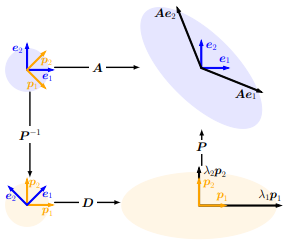
\includegraphics[width=\linewidth, height=4cm, keepaspectratio]{Pictures/maths/Eigendecomposition.png}
            \caption{Eigen Decomposition/ Eigendecomposition}
        \end{figure}
    \end{minipage}
    \hfill
    \begin{minipage}{0.68\linewidth}
        \begin{theorem}[Eigen Decomposition/ Eigendecomposition]
            A square matrix $A \in  R^{n\times n}$ can be factored into
            \[
               \hfill A = PDP^{-1} \hfill
            \]
            where $P \in  R^{n\times n}$ and $D$ is a diagonal matrix whose diagonal entries are the eigenvalues of $A$, if and only if the eigenvectors of $A$ form a basis of $R^n$.
        \end{theorem}
    \end{minipage}    
\end{table}


\begin{enumerate}
    \item \textbf{Top-left to bottom-left}: $P^{-1}$ performs a basis change from the standard basis into the \textbf{eigenbasis}\indexlabel{eigenbasis}

    \item \textbf{Bottom-left to bottom-right}: $D$ performs a scaling along the remapped orthogonal eigenvectors, depicted here by a circle being stretched to an ellipse

    \item \textbf{Bottom-right to top-right}: $P$ undoes the basis change (depicted as a reverse rotation) and restores the original coordinate frame
    
\end{enumerate}

\noindent\textbf{Note}:
\begin{enumerate}
    \item Transformations are applied in \textbf{reverse order}

    \item Let $A$ be the transformation matrix of a linear mapping with respect to the standard basis $e_i$ (blue arrows). 

    \item $P^{-1}$ performs a basis change from the standard basis into the \textbf{eigenbasis}. 

    \item the diagonal $D$ scales the vectors along these axes by the eigenvalues $\lambda_i$. 

    \item $P$ transforms these scaled vectors back into the standard/ canonical coordinates yielding $\lambda_ip_i$
\end{enumerate}

\noindent\textbf{Properties}:
\begin{enumerate}
    \item Diagonal matrices $D$ can efficiently be raised to a power. Therefore, we can find a matrix power for a matrix $A \in R^{n\times n}$ via the eigenvalue decomposition (if it exists) so that 
    \[
        A^k = (PDP^{-1})^k = (PDP^{-1})\overset{k \text{ times}}{\cdots\cdots}(PDP^{-1}) = PD^kP^{-1}
    \]
    Computing $D^k$ is efficient because we apply this operation individually to any diagonal element

    \item Assume that the eigendecomposition $A = PDP^{-1}$ exists. Then:
    \[
    det(A) = det(PDP^{-1}) = det(P)det(D)det(P^{-1}) = det(D) =  
    \hfill (det(P-1) = 1 / det(P))
    \]
    allows for an efficient computation of the determinant of $A$

    \item eigenvalue decomposition requires \textbf{square matrices}

    \item if $A$ is SPD, the decomposition is called "\textbf{spectral decomposition}"\indexlabel{spectral decomposition}

    \item if $\lambda _i$ are eigenvalues of $A$, then $\lambda _i^n$ is eigenvalues of $A^n$
\end{enumerate}


\subsection{Singular Value Decomposition (SVD) ( $A = U\Sigma V^{-1} = U\Sigma V^\top$ )}

\begin{table}[h]
    \begin{minipage}[b]{0.49\linewidth}
        \begin{figure}[H]
            \centering
            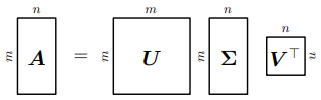
\includegraphics[width=\linewidth, height=4cm, keepaspectratio]{Pictures/maths/svd-1.png}
            \caption{SVD: Matrix Form}
        \end{figure}
    \end{minipage}
    \hfill
    \begin{minipage}[b]{0.49\linewidth}
        \begin{figure}[H]
            \centering
            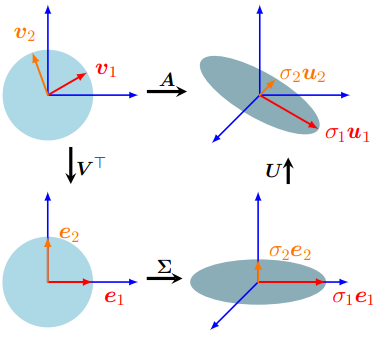
\includegraphics[width=\linewidth, height=4cm, keepaspectratio]{Pictures/maths/svd-2.png}
            \caption{SVD: Transformations}
        \end{figure}
    \end{minipage}
\end{table}

\begin{theorem}[SVD Theorem]
    Let $A \in R^{m\times n}$ be a rectangular matrix of rank $r \in [0, \min(m, n)]$. The SVD of $A$ is a decomposition of the form: $A = U\Sigma V^\top$
\end{theorem}

\begin{enumerate}
    \item \textbf{Top-left to bottom-left}: $V^\top$ performs a basis change in $R^2$ 

    \item \textbf{Bottom-left to bottom-right}: $\Sigma$ scales and maps from $R^2$ to $R^3$. The ellipse in the bottom-right lives in $R^3$. The third dimension is orthogonal to the surface of the elliptical disk.

    \item \textbf{Bottom-right to top-right}: $U$ performs a basis change within $R^3$.
\end{enumerate}

\noindent\textbf{Note}: Transformations are applied in \textbf{reverse order}

\subsubsection{Geometric Interpretation}
$\Phi : R^n \to R^m$\\

\textbf{standard bases}:\\
$B, \tilde{B} \in R^n$\\
$C, \tilde{C} \in R^m$

\vspace{0.2cm}
\noindent The SVD of a matrix can be interpreted as a decomposition of a corresponding linear mapping $\Phi  : R^n \to R^m$ into 3 operations: 
\begin{enumerate}
    \item the SVD performs a basis change via $V^\top $ 

    \begin{enumerate}
        \item scaling and augmentation (or reduction) in dimensionality via the singular value matrix $\Sigma $
    
        \item it performs a second basis change via $U$
    
        \item $V^\top  = V^{-1}$ performs a basis change from $B$ to $\tilde{B}$
    \end{enumerate}

    \item $\Sigma$  scales the new coordinates by the singular values $\Sigma _i$ (and adds or deletes dimensions), i.e., $\Sigma$  is the transformation matrix of $\Phi$  with respect to $\tilde{B}$ and $\tilde{C}$

    \item $U$ performs a basis change in the codomain $R^m$ from $\tilde{C}$ into the canonical basis of $R^m$
\end{enumerate}


\vspace{0.2cm}
\noindent\textbf{Matrix Wise analysis}

\begin{enumerate}
    \item $U \in  R^{m\times m}$ with column vectors $u_i, i = 1, \cdots  , m$
    \begin{enumerate}
        \item orthogonal matrix (SEE: \fullref{Orthogonal Matrix})

        \item $u_i$ are called the \textbf{left-singular vectors}\indexlabel{left-singular vectors}

        \item orthonormal basis $U = (u_1, \cdots  ,u_m)$ of the codomain $R^m$
    \end{enumerate}

    \vspace{0.2cm}
    \item $V \in  R^{n\times n}$ with column vectors $v_j, j = 1, \cdots  , n$
    \begin{enumerate}
        \item orthogonal matrix (SEE: \fullref{Orthogonal Matrix})

        \item $v_j$ are called the \textbf{right-singular vectors}\indexlabel{right-singular vectors}

        \item orthonormal basis $V = (v_1, \cdots  , v_n)$ of the domain $R^n$
    \end{enumerate}

    \vspace{0.2cm}
    \item $\Sigma  \in  R^{m\times n}$ with $\Sigma _{ii} = \sigma _i \geq  0$ and $\Sigma _{ij} = 0, i \neq j$
    \begin{enumerate}
        \item diagonal entries $\sigma _i, i = 1, \cdots  , r$, of $\Sigma$  are called the \textbf{singular values}\indexlabel{singular values}

        \item By convention, the singular values are ordered, i.e., $\sigma _1 \geq  \sigma _2 \geq  \sigma _r \geq  0$.

        \item it is \textbf{unique}

        \item $\Sigma$  has a \textbf{diagonal submatrix} that contains the singular values and needs additional zero padding
        \begin{enumerate}
            \item if $m > n$, then the matrix $\Sigma$  has diagonal structure up to row n and then consists of $0^\top$ row vectors from $n + 1$ to $m$ below so that:
            \[
                \Sigma =
                \begin{bmatrix}
                    \sigma_1 & 0 & 0\\
                    0 & \ddots & 0\\
                    0 & 0 & \sigma_n\\
                    0 & 0 & 0\\
                    0 & \ddots & 0\\
                    0 & 0 & 0\\
                \end{bmatrix}
            \]
    
            \item If $m < n$, the matrix $\Sigma$  has a diagonal structure up to column m and columns that consist of $0$ from $m + 1$ to $n$:
            \[
                \Sigma =
                \begin{bmatrix}
                    \sigma_1 & 0 & 0 & 0 & 0 & 0 \\
                    0 & \ddots & 0 & 0 & \ddots & 0\\
                    0 & 0 & \sigma_n & 0 & 0 & 0\\
                \end{bmatrix}
            \]
        \end{enumerate}
    \end{enumerate}
   
\end{enumerate}


\subsubsection{Constructing SVD}
\begin{enumerate}
    \item If $A$ is SPD:
    \begin{enumerate}
        \item Perform \textbf{Spectral decomposition} (SEE: \fullref{Eigen Decomposition/ Eigendecomposition})
        \[
            A = A^\top = PDP^{-1} = PDP^\top
        \]


        \item $A = U\Sigma V^\top$

        \item $\hfill U = P = V \hfill D = \Sigma \hfill$
    \end{enumerate}

    \item General $A \in R^{m\times n}$:
    \begin{enumerate}
        \item \textbf{Getting right-singular matrix (V):}
        \begin{enumerate}
            \item construct a SPD matrix $A^\top A \in R^{n\times n}$
            \[
                A^\top A = PDP^\top = P \begin{bmatrix}
                    \lambda_1 & \cdots & 0 \\
                    \vdots & \ddots & \vdots \\
                    0 & \cdots & \lambda_n\\
                \end{bmatrix} P^\top
            \]

            \item $P$ : orthogonal matrix, which is composed of the orthonormal eigenbasis

            \item $\lambda_i \geq 0$ : eigenvalues of $A^\top A$

            \item \begin{align*}
                A^\top A 
                &= (U\Sigma V^\top )^\top (U\Sigma V^\top ) \\
                &= V\Sigma ^\top U^\top U\Sigma V^\top \\
                &= V\Sigma ^\top \Sigma V^\top  &&& (U^\top U = I)\\
                &= V \begin{bmatrix}
                    \sigma_1^2 & \cdots & 0 \\
                    \vdots & \ddots & \vdots \\
                    0 & \cdots & \sigma_n^2\\
                \end{bmatrix} V^\top
            \end{align*}

            \item $V^\top = P^\top \Rightarrow V = P$

            \item $\sigma _i^2 = \lambda_i$\\
            eigenvalues of $A^\top A$ are the squared singular values of $\sigma$ 

        \end{enumerate}

        \vspace{0.2cm}
        \item \textbf{Getting left-singular matrix (U):}
        \begin{enumerate}
            \item construct a SPD matrix $AA^\top \in R^{m\times m}$
            
            \item \begin{align*}
                AA^\top 
                &= (U\Sigma V^\top )(U\Sigma V^\top )^\top \\
                &= U\Sigma V^\top V\Sigma^\top U^\top  \\
                &= U\Sigma \Sigma^\top U^\top  &&& (V^\top V = I) \\
                &= U \begin{bmatrix}
                    \sigma_1^2 & \cdots & 0 \\
                    \vdots & \ddots & \vdots \\
                    0 & \cdots & \sigma_m^2\\
                \end{bmatrix} U^\top
            \end{align*}

            \item $U^\top = P^\top \Rightarrow  U = P$
     
            \item $\sigma_j^2 = \lambda_j$
     
            \item eigenvalues of $AA^\top$ are the squared singular values of $\Sigma$

            \item \( \displaystyle u_i = \dfrac{Av_i}{||Av_i||} = \dfrac{Av_i}{\sqrt{\lambda_i}} = \dfrac{Av_i}{\sigma_i} \)

            \item \textbf{singular value equation}\indexlabel{singular value equation}: $ Av_i = \sigma_iu_i  \hfill (i = 1, \cdots , r)$
        \end{enumerate}

        \vspace{0.5cm}
        \item \textbf{Getting singular value matrix ($\Sigma$):}
        \begin{enumerate}
            \item $A^\top A$ and $AA^\top$ have \textbf{same} eigenvalues

            \vspace{0.5cm}
            \textbf{Proof}:
            \item $AA^\top x = \lambda x \Rightarrow A^\top A(A^\top x) = A^\top \lambda x = \lambda (A^\top x)$

            \item inner product between $Av_i$ and $Av_j$ must be $0$ for $i \neq j$
            \[
                (Av_i)^\top(Av_j) = v_i^\top (A^\top A)v_j = v_i^\top(\lambda_jv_j) = \lambda_jv_i^\top v_j = 0
            \]

            \item For the case $m \geq r$, it holds that $\dCurlyBrac{Av_1, \cdots , Av_r}$ is a basis of an $r$-dimensional subspace of $R^m$

            \item For $n < m$, Singular value equation holds only for $i \leq  n$, but Singular value equation says nothing about the $u_i$ for $i > n$

            \item for $m < n$, Singular value equation holds only for $i \leq  m$. For $i > m$, we have $Av_i = 0$ and we still know that the $v_i$ form an orthonormal set

            \item (\textbf{Full SVD})\indexlabel{Full SVD} For convenience in notation and abstraction, we use an SVD notation where the SVD is described as having two square left- and right-singular vector matrices, but a non-square singular value matrix. This definition for the SVD is sometimes called the \textbf{full SVD}.

            \item (\textbf{Reduced SVD})\indexlabel{Reduced SVD} SVD can be defined a bit differently and focus on square singular matrices. Then, for $A \in R^{m\times n}$ and $m \geq n$
            \[
                \hfill
                A = U\Sigma V^\top
                \hfill
                A \in  R^{m\times n}
                \hfill
                U \in  R^{m\times n}
                \hfill
                \Sigma  \in  R^{n\times n}
                \hfill
                V \in  R^{n\times n}
                \hfill
            \]

            \item (\textbf{Truncated SVD})\indexlabel{Truncated SVD} TODO

            \item It is possible to define the SVD of a rank-$r$ matrix $A$ so that $U$ is an $m\times r$ matrix, $\Sigma$  a diagonal matrix $r\times r$, and $V$ an $r\times n$ matrix. This construction is very similar to our definition, and ensures that the diagonal matrix $\Sigma$  has only nonzero entries along the diagonal. The main convenience of this alternative notation is that $\Sigma$  is diagonal, as in the eigenvalue decomposition.

            \item Restriction that the SVD for $A$ only applies to $m \times  n$ matrices with m > n is practically unnecessary. When $m < n$, the SVD decomposition will yield $\Sigma$  with more zero columns than rows and, consequently, the singular values $\sigma _{m+1}, \cdots ,\sigma _{n}$ are $0$

            
        \end{enumerate}

        
    \end{enumerate}


\end{enumerate}

\subsubsection{Properties}
\begin{enumerate}
    \item The SVD exists for any matrix $A \in R^{m\times n}$

    \item SVD expresses a change of basis in both the domain and codomain

    \item SVD also supplies an orthonormal basis of the kernel (null space) of $A$, the set of vectors $x$ with $Ax = 0$

    \item Of all possible projections, the SVD minimizes the rank-$k$ approximation error (with respect to the spectral norm) between $A$ and any rank-$k$ approximation \indexlabel{matrix: rank-k approximation}
\end{enumerate}



\subsubsection{SVD Example}
\[
    A = \begin{bmatrix}
        1 & 0 & 1 \\
        -2 & 1 & 0 \\
    \end{bmatrix}
\]

\begin{enumerate}
    \item \textbf{Right-singular vectors as the eigenbasis of $A^\top A$}
    \[
        A^\top A = 
        \begin{bmatrix}
            1 & -2 \\
            0 & 1 \\
            1 & 0 \\
        \end{bmatrix} 
        \begin{bmatrix}
            1 & 0 & 1 \\
            -2 & 1 & 0 \\
        \end{bmatrix}
        =
        \begin{bmatrix}
            5 & -2 & 1 \\
            -2 & 1 & 0 \\
            1 & 0 & 1 \\
        \end{bmatrix}
    \]


    \[
        \renewcommand{\arraystretch}{2}
        A A^\top = 
        \begin{bmatrix}
            5 & -2 & 1 \\
            -2 & 1 & 0 \\
            1 & 0 & 1 \\
        \end{bmatrix}
        =
        \begin{bmatrix}
            \dfrac{5}{\sqrt{30}} & 0 & -\dfrac{1}{\sqrt{6}} \\
            -\dfrac{2}{\sqrt{30}} & \dfrac{1}{\sqrt{5}} & -\dfrac{2}{\sqrt{6}} \\
            \dfrac{1}{\sqrt{30}} & \dfrac{2}{\sqrt{5}} & \dfrac{1}{\sqrt{6}} \\
        \end{bmatrix}
        \begin{bmatrix}
            6 & 0 & 0\\
            0 & 1 & 0 \\
            0 & 0 & 0 \\
        \end{bmatrix}
        \begin{bmatrix}
            \dfrac{5}{\sqrt{30}} & -\dfrac{2}{\sqrt{30}} & \dfrac{1}{\sqrt{30}} \\
            0 & \dfrac{1}{\sqrt{5}} & \dfrac{2}{\sqrt{5}} \\
            -\dfrac{1}{\sqrt{6}} & -\dfrac{2}{\sqrt{6}} & \dfrac{1}{\sqrt{6}}
        \end{bmatrix}
        = PDP^\top
    \]

    \[
        \renewcommand{\arraystretch}{2}
        V = P =
        \begin{bmatrix}
            \dfrac{5}{\sqrt{30}} & 0 & -\dfrac{1}{\sqrt{6}} \\
            -\dfrac{2}{\sqrt{30}} & \dfrac{1}{\sqrt{5}} & -\dfrac{2}{\sqrt{6}} \\
            \dfrac{1}{\sqrt{30}} & \dfrac{2}{\sqrt{5}} & \dfrac{1}{\sqrt{6}} \\
        \end{bmatrix}
    \]

    \vspace{0.5cm}
    \item \textbf{Singular-value matrix:}\\
    As the singular values $\sigma _i$ are the square roots of the eigenvalues of $A^\top A$ we obtain them straight from $D$. Since $rk(A) = 2$, there are only two nonzero singular values: $\sigma _1 = \sqrt{6}$ and $\sigma _2 = 1$.
    \[
        \Sigma = 
        \begin{bmatrix}
            \sqrt{6} & 0 & 0 \\
            0 & 1 & 0 \\
            0 & 0 & 0 \\
        \end{bmatrix}
    \]

    \vspace{0.5cm}
    \item \textbf{Left-singular vectors as the normalized image of the right-singular vectors}
    \[
        \hfill
        \renewcommand{\arraystretch}{2}
        u_1 = \dfrac{Av_1}{\sigma_1} = \dfrac{1}{\sqrt{6}} 
        \begin{bmatrix}
            1 & 0 & 1 \\
            -2 & 1 & 0 \\
        \end{bmatrix}
        \begin{bmatrix}
            \dfrac{5}{\sqrt{30}} \\
            -\dfrac{2}{\sqrt{30}} \\
            \dfrac{1}{\sqrt{30}} \\
        \end{bmatrix}
        = 
        \begin{bmatrix}
            \dfrac{1}{\sqrt{5}} \\
            -\dfrac{2}{\sqrt{5}}
        \end{bmatrix}
        \hspace{0.5cm}
        \renewcommand{\arraystretch}{2}
        u_2 = \dfrac{Av_2}{\sigma_2} = \dfrac{1}{1} 
        \begin{bmatrix}
            1 & 0 & 1 \\
            -2 & 1 & 0 \\
        \end{bmatrix}
        \begin{bmatrix}
            0 \\
            \dfrac{1}{\sqrt{5}} \\
            \dfrac{2}{\sqrt{5}} \\
        \end{bmatrix}
        = 
        \begin{bmatrix}
            \dfrac{2}{\sqrt{5}} \\
            \dfrac{1}{\sqrt{5}}
        \end{bmatrix}
        \hfill
    \]
    \[
        \renewcommand{\arraystretch}{2}
        U = [u_1, u_2] = 
        \begin{bmatrix}
            \dfrac{1}{\sqrt{5}} & \dfrac{2}{\sqrt{5}} \\
            -\dfrac{2}{\sqrt{5}} & \dfrac{1}{\sqrt{5}} \\
        \end{bmatrix}
        = 
        \dfrac{1}{\sqrt{5}}
        \begin{bmatrix}
            1 & {2} \\
            -{2} & {1} \\
        \end{bmatrix}
    \]
    
\end{enumerate}


\subsection{Eigenvalue Decomposition vs. Singular Value Decomposition (SVD)}

\begin{table}[H]
    \begin{tabular}{l l}
        eigendecomposition & $A = PDP^{-1}$ \\
        SVD & $A = U\Sigma V^\top$
    \end{tabular}
\end{table}

\begin{enumerate}
    \item The SVD always exists for any matrix $R^{m\times n}$. The eigendecomposition is only defined for square matrices $R^{n\times n}$ and only exists if we can find a basis of eigenvectors of $R^n$

    \item The vectors in the eigendecomposition matrix $P$ are not necessarily orthogonal, i.e., the change of basis is not a simple rotation and scaling. On the other hand, the vectors in the matrices $U$ and $V$ in the SVD are orthonormal, so they do represent rotations

    \item Both the eigendecomposition and the SVD are compositions of three linear mappings:

    \begin{enumerate}
        \item Change of basis in the domain
    
        \item Independent scaling of each new basis vector and mapping from domain to codomain
    
        \item Change of basis in the codomain
    \end{enumerate}

    \item A key difference between the eigendecomposition and the SVD is that in the SVD, domain and codomain can be vector spaces of different dimensions

    \item In the SVD, the left- and right-singular vector matrices $U$ and $V$ are generally not inverse of each other (they perform basis changes in different vector spaces). In the eigendecomposition, the basis change matrices $P$ and $P^{-1}$ are inverses of each other.

    \item In the SVD, the entries in the diagonal matrix $\Sigma$ are all real and nonnegative, which is not generally true for the diagonal matrix in the eigendecomposition

    \item The SVD and the eigendecomposition are closely related through their projections:
    \begin{enumerate}
        \item The left-singular vectors of $A$ are eigenvectors of $AA^\top$ 
    
        \item The right-singular vectors of $A$ are eigenvectors of $A^\top A$
    
        \item The nonzero singular values of $A$ are the square roots of the nonzero eigenvalues of both $AA^\top$  and $A^\top A$
    \end{enumerate}

    \item For symmetric matrices $A \in  R^{n\times n}$ , the eigenvalue decomposition and the SVD are one and the same (using spectral theorem)

\end{enumerate}



\subsection{LU decomposition ( $A = LU$ ) \cite{wiki/LU_decomposition}} \label{LU decomposition}

\subsubsection{General}
\[
    \displaystyle 
    \begin{bmatrix}
        a_{11} & a_{12} & a_{13} \\
        a_{21} & a_{22} & a_{23}\\
        a_{31} & a_{32} & a_{33}
    \end{bmatrix}
    =
    \begin{bmatrix}
        l _{11} & 0 & 0\\
        l _{21} & l _{22} & 0\\
        l _{31} & l _{32} & l _{33}
    \end{bmatrix}
    \begin{bmatrix}
        u_{11} & u_{12} & u_{13}\\
        0 & u_{22} & u_{23}\\
        0 & 0 & u_{33}
    \end{bmatrix}
\]

\subsubsection{Doolittle Decomposition}\label{LU: Doolittle Decomposition}

\[
    \displaystyle 
    \begin{bmatrix}
        a_{11} & a_{12} & a_{13} \\
        a_{21} & a_{22} & a_{23}\\
        a_{31} & a_{32} & a_{33}
    \end{bmatrix}
    =
    \begin{bmatrix}
        1 & 0 & 0\\
        l _{21} & 1 & 0\\
        l _{31} & l _{32} & 1
    \end{bmatrix}
    \begin{bmatrix}
        u_{11} & u_{12} & u_{13}\\
        0 & u_{22} & u_{23}\\
        0 & 0 & u_{33}
    \end{bmatrix}
\]

\subsubsection{Crout Decomposition}\label{LU: Crout Decomposition}

\[
    \displaystyle 
    \begin{bmatrix}
        a_{11} & a_{12} & a_{13} \\
        a_{21} & a_{22} & a_{23}\\
        a_{31} & a_{32} & a_{33}
    \end{bmatrix}
    =
    \begin{bmatrix}
        l _{11} & 0 & 0\\
        l _{21} & l _{22} & 0\\
        l _{31} & l _{32} & l _{33}
    \end{bmatrix}
    \begin{bmatrix}
        1 & u_{12} & u_{13}\\
        0 & 1 & u_{23}\\
        0 & 0 & 1
    \end{bmatrix}
\]



\section{Matrix Approximation \cite{mfml-1}}\label{Matrix Approximation}

SVD allows us to represent a matrix $A$ as a sum of simpler (low-rank) matrices $A_i$, which lends itself to a matrix approximation scheme that is cheaper to compute than the \textbf{full SVD}.

\[
    A_i := u_iv_i^\top \hfill \text{(rank-$1$ matrix $A_i \in R^{m\times n}$)}
\]

which is formed by the outer product of the $i$th orthogonal column vector of $U$ and $V$

\[
    \displaystyle
    A = 
    \sum_{i=1}^{r} \sigma_iu_iv^\top
    =
    \sum_{i=1}^{r} \sigma_iA_i
    \hfill
    (rk(A)=r)
\]
where the outer-product matrices $A_i$ are weighted by the $i$th singular value $\sigma_i$\\
All terms $\displaystyle \sum_{i=1}^{r} u_iv^\top$ vanish for $i \neq j$ because $\Sigma$ is a diagonal matrix. Any terms $i > r$ vanish because the corresponding singular values are $0$.

\vspace{0.2cm}
\textbf{rank-k approximation}:
\[
    \displaystyle
    \hat{A}(k) = 
    \sum_{i=1}^{k} \sigma_iu_iv^\top
    =
    \sum_{i=1}^{k} \sigma_iA_i
    \hfill
    (rk(\hat{A}(k))=k)
    (k < r)
\]

\begin{theorem}[Eckart-Young Theorem]\indexlabel{rank-k approximation: Eckart-Young Theorem}
    Consider a matrix $A \in R^{m\times n}$ of rank $r$ and let $B \in R^{m\times n}$ be a matrix of rank $k$. For any $k \leq r$ with $\hat{A}(k) = \sum_{i=1}^{k} \sigma_iu_iv^\top$ it holds that:
    \begin{enumerate}
        \item $\displaystyle \hat{A}(k) = \arg\min_{rk(B)=k} ||A-B||_2$

        \item $\displaystyle ||A-\hat{A}(k)||_2 = \sigma_{k+1} \hfill (\text{rank-r approximation error})$\indexlabel{rank-r approximation error}
    \end{enumerate}
\end{theorem}

\begin{enumerate}
    \item We can interpret the rank-$k$ approximation obtained with the SVD as a projection of the full-rank matrix $A$ onto a lower-dimensional space of rank-at-most-$kS$ matrices.

    \item \[
        \displaystyle
        A - \hat{A}(k) = 
        \sum_{i=k+1}^{r} \sigma_iu_iv^\top
    \]

    \item $\sigma_{k+1}$ : spectral norm of the difference matrix

    \item let matrix $B$ with $rk(B) \leq k$, such that $||A-B||_2 < ||A-\hat{A}(k)||_2$ then there exists an at least $(n - k)$-dimensional null space $Z \subseteq R^n$, such that $x \in Z$ implies that $Bx = 0$. Then it follows that $||Ax||_2=||(A-B)x||_2$ and by using a version of the Cauchy-Schwarz inequality  that encompasses norms of matrices, we obtain $||Ax||_2 \leq ||A-B||_2||x||_2 \leq \sigma_{k+1}||x||_2$

    \item there exists a $(k + 1)$-dimensional subspace where $||Ax||_2 \geq \sigma _{k+1}||x||_2$, which is spanned by the right-singular vectors $v_j, j \leq k + 1$ of $A$

    \item Adding up dimensions of these two spaces yields a number greater than $n$, as there must be a non-zero vector in both spaces. This is a \textbf{contradiction} of the \textbf{rank-nullity theorem}

    \item We can use SVD to reduce a rank-$r$ matrix $A$ to a rank-k matrix  in a principled, optimal (in the spectral norm sense) manner. We can interpret the approximation of $A$ by a rank-$k$ matrix as a form of \textbf{lossy compression}\indexlabel{rank-k approx: lossy compression}.

\end{enumerate}



\section{Gradients of Matrices}
\subsection{With Respect to Matrix}
if we compute the gradient of an $m \times  n$ matrix $A$ with respect to a $p \times  q$ matrix $B$, the resulting Jacobian would be $(m\times n)\times (p\times q)$, i.e., a four-dimensional tensor $J$, whose entries are given as $J_{ijkl} = \partial A_{ij}/\partial B_{kl}$


























